\section{Appendix}
\label{sec:appendix}

% Not counted in the 8 pages.

% A. Benchmark cases: table of the 48 main cases (id, category, request, expected size) and the 30 organic cases
%    (id, subject, request). From eval/cases.json and eval/organic_cases.json.
\subsection{Benchmark cases}
Every request in both suites, as sent to the builder.
For the main suite, each case's category, whether it should be built or declined (\emph{either}: both count), and the expected size, which is checked in any axis order.
For the organic suite, the phrase used for the Thingiverse search.
The files are generated by \texttt{python -m scripts.report\_figures appendix} from \texttt{eval/cases.json} and \texttt{eval/organic\_cases.json}.

% Made by `python -m scripts.report_figures appendix` from eval/cases.json and eval/organic_cases.json.
\subsection*{Main suite (48 cases)}
{\small
\noindent\textbf{s01} \emph{simple, build, 12\,$\times$\,12\,$\times$\,15\,mm}: A cylindrical spacer with 12mm outer diameter, 6.5mm inner diameter, 15mm long.\par
\noindent\textbf{s02} \emph{simple, build, 25\,$\times$\,25\,$\times$\,25\,mm}: A 25mm cube with a 10mm diameter hole drilled through the centre from top to bottom.\par
\noindent\textbf{s03} \emph{simple, build, 34.64\,$\times$\,30\,$\times$\,8\,mm}: A hexagonal prism 30mm across the flats and 8mm tall.\par
\noindent\textbf{s04} \emph{simple, build, 70\,$\times$\,20\,$\times$\,4\,mm}: A 70mm x 20mm x 4mm bar with a 40mm long, 6mm wide slot through it, centred along its length.\par
\noindent\textbf{s05} \emph{simple, build, 40\,$\times$\,40\,$\times$\,30\,mm}: A solid cone 40mm in base diameter and 30mm tall.\par
\noindent\textbf{m01} \emph{medium, build, 120\,$\times$\,80\,$\times$\,4\,mm}: A 120mm x 80mm x 4mm mounting plate with a 3 by 2 grid of 5mm holes spaced 30mm apart, centred on the plate, and all four corners rounded with an 8mm radius.\par
\noindent\textbf{m02} \emph{medium, build, 100\,$\times$\,60\,$\times$\,15\,mm}: An open-top rectangular tray 100mm x 60mm x 15mm with 2mm walls and a 2mm floor, with one 2mm divider wall splitting it into two equal compartments along its length.\par
\noindent\textbf{m03} \emph{medium, build, 30\,$\times$\,30\,$\times$\,15\,mm}: A round knob 30mm in diameter and 15mm tall, with a 6mm D-shaped shaft hole 10mm deep in the bottom; the flat of the D is 1mm in from the circle.\par
\noindent\textbf{m04} \emph{medium, build, 60\,$\times$\,60\,$\times$\,5\,mm}: A 60mm diameter disc, 5mm thick, with a 20mm centre hole and eight 4mm holes evenly spaced on a 45mm bolt circle.\par
\noindent\textbf{m05} \emph{medium, build, 80\,$\times$\,20\,$\times$\,5\,mm}: A cable comb: an 80mm x 20mm x 5mm bar with six 4mm wide, 12mm deep slots cut into one long edge, evenly spaced along it.\par
\noindent\textbf{m06} \emph{medium, build, 100\,$\times$\,30\,$\times$\,20\,mm}: A U-channel 100mm long, 30mm wide and 20mm tall, with 3mm thick walls and base, open at the top and both ends.\par
\noindent\textbf{m07} \emph{medium, build, 50\,$\times$\,50\,$\times$\,60\,mm}: A cylindrical cup 50mm outer diameter and 60mm tall with 2mm walls and a 2mm base, open at the top, with the outer bottom edge filleted with a 3mm radius.\par
\noindent\textbf{m08} \emph{medium, build, 40\,$\times$\,40\,$\times$\,10\,mm}: A pipe clamp ring: 10mm tall, 32mm inner diameter, 4mm wall, with a 2mm wide gap cut through one side of the ring.\par
\noindent\textbf{m09} \emph{medium, build, 50\,$\times$\,50\,$\times$\,6\,mm}: A 50mm x 50mm x 6mm plate with a 30mm square pocket, 3mm deep, centred in the top face; the pocket's four inside corners are rounded with a 4mm radius.\par
\noindent\textbf{m10} \emph{medium, build, 20\,$\times$\,20\,$\times$\,40\,mm}: A 20mm diameter pin 40mm long with a 2mm chamfer on both end edges and a 3mm wide, 1.5mm deep groove around it halfway along its length.\par
\noindent\textbf{m11} \emph{medium, build, 25\,$\times$\,40\,$\times$\,3\,mm}: A 25mm wide, 40mm tall, 3mm thick hanging plate with a keyhole cut through it: an 8mm diameter hole centred 12mm above the bottom edge, with a 4mm wide slot running 10mm straight up from the hole's centre.\par
\noindent\textbf{m12} \emph{medium, build, 25\,$\times$\,25\,$\times$\,10\,mm}: A shaft collar: 25mm outer diameter, 10mm bore, 10mm long, with a 3.3mm radial hole drilled from the outside into the bore, centred along its length.\par
\noindent\textbf{m13} \emph{medium, build, 16\,$\times$\,16\,$\times$\,60\,mm}: A stepped shaft on one axis: 10mm diameter for the first 20mm, then 16mm diameter for 15mm, then 8mm diameter for the last 25mm.\par
\noindent\textbf{m14} \emph{medium, build, 70\,$\times$\,50\,$\times$\,25\,mm}: An open-top box 60mm x 40mm x 25mm with 2mm walls and floor, with a 3mm thick flange sticking out 5mm all around the outside of the top rim, flush with the top.\par
\noindent\textbf{m15} \emph{medium, build, 15.01\,$\times$\,13\,$\times$\,35\,mm}: A bolt blank: a hexagonal head 13mm across the flats and 5mm tall, with a plain 8mm diameter shank 30mm long (no thread).\par
\noindent\textbf{m16} \emph{medium, build, 57.06\,$\times$\,54.27\,$\times$\,6\,mm}: A five-pointed star 6mm thick: the points lie on a 30mm radius circle and the inner corners on a 12mm radius circle.\par
\noindent\textbf{m17} \emph{medium, build, 100\,$\times$\,20\,$\times$\,40\,mm}: A 100mm long, 20mm deep, 40mm tall block with a 60mm diameter semicircular arch cut through it from front to back, centred on the bottom edge.\par
\noindent\textbf{h01} \emph{hard, build, 44\,$\times$\,44\,$\times$\,8\,mm}: A spur gear with 20 teeth, module 2, 8mm thick, with a 5mm centre bore.\par
\noindent\textbf{h02} \emph{hard, build, no fixed size}: A phone stand: a 70mm wide, 80mm deep, 5mm thick base plate; a 5mm thick, 90mm long back support leaning back at 65 degrees from the base; and a 10mm tall lip along the front edge to stop the phone sliding.\par
\noindent\textbf{h03} \emph{hard, build, no fixed size}: A wall hook: a 40mm x 60mm x 5mm back plate with two 4mm countersunk screw holes, and a curved hook arm that sticks out 35mm from the lower part of the plate and curves upward at the end.\par
\noindent\textbf{h04} \emph{hard, build, 40\,$\times$\,40\,$\times$\,12\,mm}: A pulley wheel 40mm in diameter and 12mm wide with an 8mm bore and a V-groove around its rim, 6mm wide at the surface and 4mm deep.\par
\noindent\textbf{h05} \emph{hard, build, 20\,$\times$\,20\,$\times$\,32\,mm}: A coil spring made from 2mm diameter round wire: 20mm outer diameter, 5 turns at a 6mm pitch.\par
\noindent\textbf{h06} \emph{hard, build, 60\,$\times$\,60\,$\times$\,23\,mm}: A desk cable grommet: a 60mm diameter, 3mm thick round flange on top of a 50mm outer diameter, 20mm long tube with 2mm walls, open through the middle, with a 15mm wide slot cut through the flange and tube from one side to the centre so a cable can be slipped in.\par
\noindent\textbf{h07} \emph{hard, build, 40\,$\times$\,40\,$\times$\,20\,mm}: A 90 degree pipe elbow: a tube with 20mm outer and 16mm inner diameter, bent through 90 degrees around a 30mm centreline radius, with no straight ends.\par
\noindent\textbf{h08} \emph{hard, build, 80\,$\times$\,60\,$\times$\,5\,mm}: An 80mm x 60mm x 5mm honeycomb panel: a grid of hexagonal through-holes 8mm across the flats with 2mm walls between them, leaving a solid border at least 3mm wide around the edge.\par
\noindent\textbf{h09} \emph{hard, build, 25\,$\times$\,25\,$\times$\,90\,mm}: A tool handle 25mm in diameter and 90mm long overall, with a fully rounded hemispherical back end and six 4mm diameter half-round flutes running along the straight part, evenly spaced around it.\par
\noindent\textbf{h10} \emph{hard, build, 60\,$\times$\,50\,$\times$\,40\,mm}: An L-bracket 50mm wide with a 60mm long horizontal leg and a 40mm tall vertical leg, both 5mm thick, braced by two 5mm thick triangular gussets flush with the side edges, with two 5mm holes in each leg.\par
\noindent\textbf{h11} \emph{hard, build, 80\,$\times$\,80\,$\times$\,70\,mm}: A tapered square planter 70mm tall, 60mm square at the bottom and 80mm square at the top, with 3mm walls and base, open at the top, and a 10mm drainage hole in the centre of the base.\par
\noindent\textbf{h12} \emph{hard, build, 40\,$\times$\,40\,$\times$\,10\,mm}: A thumbwheel 40mm in diameter and 10mm thick with 30 semicircular 2mm diameter notches evenly spaced around its rim and a hexagonal socket 5mm across the flats through the centre.\par
\noindent\textbf{h13} \emph{hard, build, 60\,$\times$\,40\,$\times$\,30\,mm}: An open-top box 60mm x 40mm x 30mm with 2mm walls and floor, with a 1.5mm tall, 1mm deep groove cut into the inside of both long walls, 3mm below the top edge, for a sliding lid.\par
\noindent\textbf{p01} \emph{casual, build, 150\,$\times$\,25\,$\times$\,3\,mm}: Make me a ruler with my name engraved on it. The ruler is 150mm long, 25mm wide and 3mm thick, with the name ALEX engraved 0.5mm deep and a tick mark every 10mm along one long edge.\par
\noindent\textbf{p02} \emph{casual, either, no fixed size}: Make a die that has 2 snakes and 4 ladders instead of numbers.\par
\noindent\textbf{p03} \emph{casual, decline}: Create a tree that has a cat on it.\par
\noindent\textbf{p04} \emph{casual, decline}: A realistic, anatomically accurate model of a human hand.\par
\noindent\textbf{p05} \emph{casual, either, no fixed size}: A chess knight.\par
\noindent\textbf{p06} \emph{casual, build, 25\,$\times$\,25\,$\times$\,40\,mm}: A chess rook 40mm tall and 25mm across at its widest point (the base), with a castle top that has four notches cut into its rim.\par
\noindent\textbf{p07} \emph{casual, decline}: A bust of Abraham Lincoln.\par
\noindent\textbf{p08} \emph{casual, either, no fixed size}: A low-poly fox figurine about 60mm tall.\par
\noindent\textbf{c01} \emph{casual, build, 80\,$\times$\,40\,$\times$\,25\,mm}: Can you make me something to stand my AA batteries up in? 8 of them in two rows of four, holes 15mm wide and 20mm deep, in an 80 x 40 x 25 block.\par
\noindent\textbf{c02} \emph{casual, build, 50\,$\times$\,30\,$\times$\,20\,mm}: I need a little open tray to keep SD cards in. It has to fit a 50 x 30 x 20mm spot on my shelf, thin walls are fine.\par
\noindent\textbf{c03} \emph{casual, build, no fixed size}: something to prop my 70mm wide phone up at an angle on my desk\par
\noindent\textbf{c04} \emph{casual, build, no fixed size}: My table leg is a 25mm round tube and it scratches the floor. Make a cap that slides 15mm onto the end, with a 3mm thick bottom.\par
\noindent\textbf{c05} \emph{casual, build, no fixed size}: a hook that screws to the underside of my desk so I can hang my headphones on it\par
}
\subsection*{Organic suite (30 cases)}
{\small
\noindent\textbf{o01} \emph{search: sitting cat}: A sitting cat about 50 mm tall, tail curled around its front paws, ears pointing up.\par
\noindent\textbf{o02} \emph{search: horse figurine}: A standing horse figurine, 60 mm tall, four legs, long neck and head raised, a tail hanging down.\par
\noindent\textbf{o03} \emph{search: frog}: A frog sitting on its folded back legs, about 40 mm long, with big bulging eyes on top of its head.\par
\noindent\textbf{o04} \emph{search: tulip flower}: A tulip flower 80 mm tall: a cup-shaped bloom of petals on a straight stem with two long leaves, on a small round base.\par
\noindent\textbf{o05} \emph{search: octopus}: A cartoon octopus 50 mm tall: a round head and eight curling tentacles spread around it on the ground.\par
\noindent\textbf{o06} \emph{search: owl figurine}: An owl figurine 50 mm tall: an egg-shaped body, a round face with two large eyes and a small beak, ear tufts, wings folded at the sides.\par
\noindent\textbf{o07} \emph{search: rubber duck}: A rubber duck, 45 mm tall, with a flat bottom so it stands.\par
\noindent\textbf{o08} \emph{search: brontosaurus}: A long-necked dinosaur (brontosaurus) 80 mm long: a heavy body on four pillar legs, a long neck with a small head, and a long tail.\par
\noindent\textbf{o09} \emph{search: hand sculpture}: A human hand, palm open with fingers spread, standing upright on its wrist, 90 mm tall.\par
\noindent\textbf{o10} \emph{search: apple fruit}: An apple 50 mm wide with a short stem and one leaf.\par
\noindent\textbf{o11} \emph{search: dolphin}: A dolphin leaping in an arc, 70 mm long, with a dorsal fin, flippers and a tail fluke, the tail touching a small round base.\par
\noindent\textbf{o12} \emph{search: turtle}: A turtle 60 mm long: a domed shell, four stubby legs, a head poking out the front and a short tail.\par
\noindent\textbf{o13} \emph{search: seahorse}: A seahorse 70 mm tall, upright, with a curled tail touching a small round base, a long snout and a ridged belly.\par
\noindent\textbf{o14} \emph{search: crab}: A crab 60 mm wide: a flat oval shell, two raised claws at the front, four legs on each side, and eyes on short stalks.\par
\noindent\textbf{o15} \emph{search: starfish}: A starfish 70 mm across with five thick arms tapering to rounded tips, lying flat, with a bumpy top.\par
\noindent\textbf{o16} \emph{search: shark figurine}: A shark 80 mm long, swimming, on a small stand: a pointed snout, a tall dorsal fin, two side fins and a forked tail.\par
\noindent\textbf{o17} \emph{search: walrus}: A walrus 55 mm tall, resting on its belly with its front flippers on the ground, a round head, whiskered snout and two long tusks pointing down.\par
\noindent\textbf{o18} \emph{search: chicken figurine}: A chicken 50 mm tall standing on two legs, a round body, a comb on top of its head, a small beak and tail feathers raised at the back.\par
\noindent\textbf{o19} \emph{search: llama}: A standing llama 75 mm tall: four thin legs, a long upright neck, a small head with tall pointed ears and a fluffy body.\par
\noindent\textbf{o20} \emph{search: parrot figurine}: A parrot 60 mm tall perched upright on a short branch, with a curved hooked beak, folded wings and a long tail hanging down.\par
\noindent\textbf{o21} \emph{search: pineapple}: A pineapple 80 mm tall: an oval fruit with a criss-cross scaled surface and a crown of spiky leaves on top.\par
\noindent\textbf{o22} \emph{search: banana}: A single banana 90 mm long, curved, with a short stem at one end, lying on its side.\par
\noindent\textbf{o23} \emph{search: strawberry}: A strawberry 40 mm tall, heart-shaped, with small seed dimples over its surface and a crown of leaves on top.\par
\noindent\textbf{o24} \emph{search: avocado half}: Half an avocado 70 mm long, cut side up, lying flat, with the round pit sitting in the middle.\par
\noindent\textbf{o25} \emph{search: garlic bulb}: A garlic bulb 45 mm tall: plump cloves bulging around a rounded base, gathered into a pointed tip at the top.\par
\noindent\textbf{o26} \emph{search: rose flower}: A single rose 90 mm tall: a tight spiral bloom of petals on a straight stem with two leaves, on a small round base.\par
\noindent\textbf{o27} \emph{search: palm tree}: A palm tree 90 mm tall: a slightly curved ringed trunk on a small round base, with long drooping fronds spreading from the top.\par
\noindent\textbf{o28} \emph{search: molar tooth}: A molar tooth 40 mm tall, standing on its two roots, with a wide crown and a bumpy top.\par
\noindent\textbf{o29} \emph{search: croissant}: A croissant 80 mm long, crescent-shaped, with rolled layers that swell in the middle and taper to the two curved ends.\par
\noindent\textbf{o30} \emph{search: cupcake}: A cupcake 50 mm tall: a ridged paper cup, a swirl of frosting on top and a cherry at the peak.\par
}


% B. Prompts: build prompt (generate.py SYSTEM_PROMPT), SDF prompt (SYSTEM_PROMPT_SDF, maybe shortened), judge
%    prompt (judge/prompts/<version>.txt).
\subsection{Prompts}
The system prompts used in the round: for CadQuery builds, for SDF sculpting, and for the visual judge (version 2, paired with the render with a flat bottom view).
The request, and with RAG the retrieved examples, go in the first user message after it.

\paragraph{Build prompt (CadQuery).}
\lstinputlisting{appendix/prompt_build.txt}

\paragraph{Sculpting prompt (SDF).}
\lstinputlisting{appendix/prompt_sdf.txt}

\paragraph{Judge prompt.}
\lstinputlisting{appendix/prompt_judge.txt}

% C. Per-category results (report-v1.md "Per model and category"), full results table, failure-type table,
%    pass@k table, time table if not in the main text.
\subsection{How the main-suite runs ended}
Table~\ref{tab:outcomes} counts how each builder's runs of the 42 cases that should be built ended (3 runs each, 126 per builder, with RAG).

\begin{table}[h]
  \centering
  \small
  \setlength{\tabcolsep}{3pt}
  \begin{tabular}{@{}lccccc@{}}
    \toprule
    & Right & Wrong & Wrong & \multicolumn{2}{c}{No part} \\
    \cmidrule(l){5-6}
    Builder & part & shape & size & Script & Other \\
    \midrule
    Sonnet 5.5     & 124 & 0  & 2  & 0   & 0  \\
    Haiku 5.5      & 118 & 8  & 0  & 0   & 0  \\
    Gemini 3.5 FL  & 89  & 20 & 3  & 6   & 8  \\
    Gemma 4 31B    & 102 & 11 & 0  & 8   & 5  \\
    Gemma 4 12B    & 65  & 30 & 1  & 17  & 13 \\
    Qwen 4B FT     & 38  & 29 & 10 & 28  & 21 \\
    Qwen 4B        & 9   & 5  & 3  & 101 & 8  \\
    \bottomrule
  \end{tabular}
  \caption{How the runs of the 42 build cases ended. \emph{Right part}: right size and passed by the judge.
    \emph{Wrong shape}: right size, failed by the judge. \emph{No part}: the last attempt failed with a script error,
    or otherwise (the mesh check failed, no code, or the reply was cut off). FL: Flash Lite; FT: fine-tuned.}
  \label{tab:outcomes}
\end{table}

% D. More renders: a sheet of example parts per model, good and bad.
\subsection{What the judge sees}
Fig.~\ref{fig:judge} shows a full render as the judge receives it, for a correct part and for a part of the right size without its holes.

% Figure: renders copied by `pixi run -e cap6938 python -m scripts.report_figures judge-example`, which also prints
% the judge's replies quoted below (gemini-3.8-flash, report-v1, same verdict in all 3 runs).
\begin{figure*}[h]
  \centering
  \small
  \textit{``Can you make me something to stand my AA batteries up in? 8 of them in two rows of four, holes 15mm wide
    and 20mm deep, in an 80 x 40 x 25 block.''}\\[4pt]
  \begin{minipage}[t]{0.485\linewidth}
    \centering
    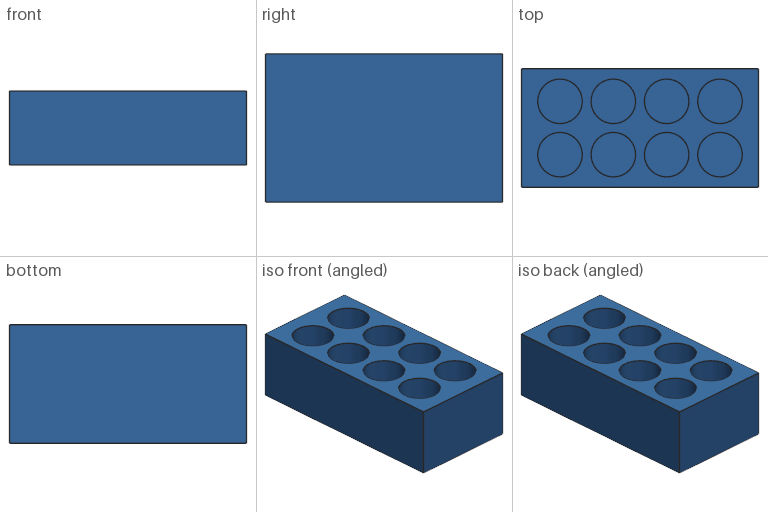
\includegraphics[width=\linewidth]{figures/judge_c01_reference.png}\\[2pt]
    (a) Reference solution: score 1.0 (\emph{pass}).
  \end{minipage}\hfill
  \begin{minipage}[t]{0.485\linewidth}
    \centering
    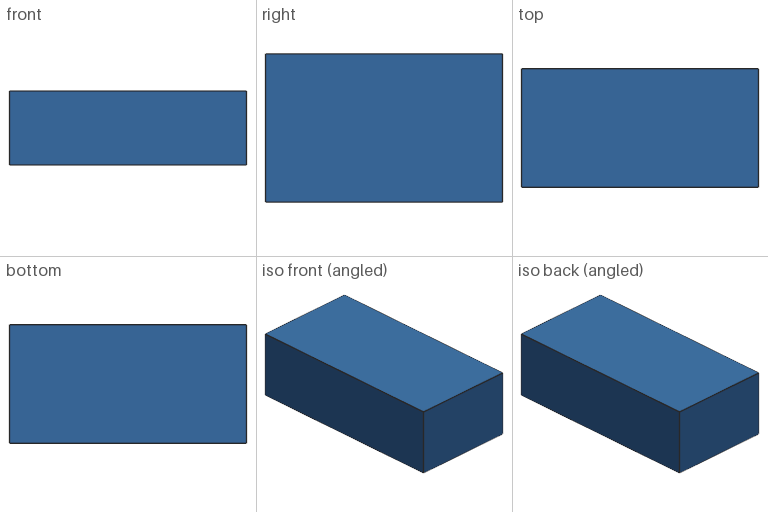
\includegraphics[width=\linewidth]{figures/judge_c01_gemma31b.png}\\[2pt]
    (b) Gemma 4 31B build: score 0.11 (\emph{fail}). ``Missing all 8 holes for the AA batteries; part is a
    completely solid block.''
  \end{minipage}
  \caption{What the visual judge sees: six views of the part (four flat, two angled), sent in one request with the
    request text and the measured size. Both parts measure $80 \times 40 \times 25$\,mm, so the size check accepts
    both; only the top and angled views show that (b) has no holes. The judge scores 1--10 on four bands (match,
    small deviations, a feature wrong, a different object), rescaled to 0--1; 0.5 and above passes. It gave each part
    the same score in all 3 runs, and the hand grade for (b) is ``different object''.}
  \label{fig:judge}
\end{figure*}

\subsection{Renders}
The renders of every judged part are kept in \texttt{eval/renders/}, and \texttt{judge sheet --study report-v1} builds a page that shows them side by side with the judge's score and reasons.

% E. Spend and hardware (report-v1.md "Spend"; study header).
\subsection{Spend and hardware}
The round cost \$8.58 at Anthropic: \$3.80 for builds (Sonnet \$3.21, Haiku \$0.59) and \$4.78 for judging (Sonnet \$4.55, Haiku \$0.22, checks \$0.01).
At Google, Gemini 3.5 Flash Lite's builds cost \$1.36 and judging with Gemini 3.1 Flash Lite \$0.79.
Gemini 3.8 Flash (judging, 2.5M input and 114K output tokens) and Gemma 4 31B (builds) have no listed price.
Local models ran in Ollama with a 16K-token context on one NVIDIA RTX 3080 (10\,GB), for about 36 hours of GPU time.
